\chapter{Searching for Homomorphisms}
\label{chap:hf}

In this chapter, we explore spatial homomorphisms in continuous domains.
We begin by describing the challenges of such a definition
(\secref{sec:hf:continuous-hom}), and describe a extension to existing
MDP homomorphism definitions that tackles them
(\secref{sec:hf:definition}). As an aside, we detail an interesting
family of continuous homomorphisms, namely continuous affine
homomorphisms in \secref{sec:hf:affine}. We develop an online algorithm
to find homomorphisms from this family in
\secref{sec:hf:homomorphic-filters}, and evaluate this algorithm in
\secref{sec:hf:experiments}.

\section{Continuous Homomorphisms}
\label{sec:hf:continuous-hom}

An important property of symmetries in continuous domains is that they
may reduce the dimensionality of the domain; the type of symmetries
present in discrete domains can only ``fold'' the state space in
finitely many ways. To motivate this distinction, consider the following
examples,

\begin{figure}[h]
  \centering
  \subfloat[Discrete Symmetry]{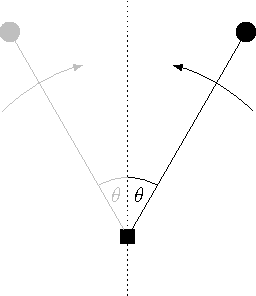
\includegraphics[width=2in]{figures/inverted-pendulum} \label{fig:inverted-pendulum}} \hspace{0.5in} 
  \subfloat[Continuous Symmetry]{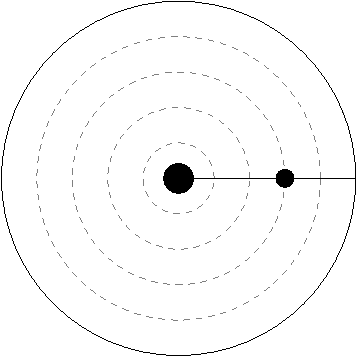
\includegraphics[width=2in]{figures/reach-center} \label{fig:reach-center}} 
%  \subfloat[Octopus Arm: Algebraic (Continuous) Symmetry]{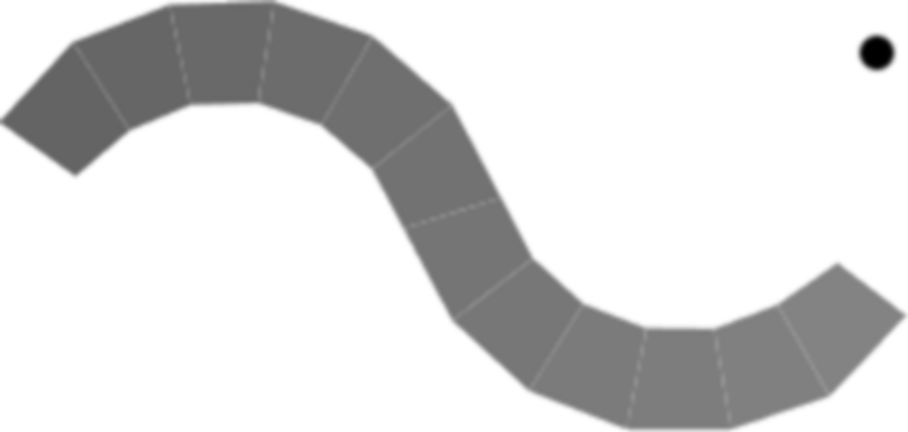
\includegraphics[width=6cm]{figures/octopus} \label{fig:octopus}}
\end{figure}

\subsection{Inverted Pendulum} 
In this example, the agent is aware of a single continuous variable,
the angular displacement of the pole from the vertical, and has either
two discrete actions to move to the left or to the right with
a certain acceleration/impulse, or a continuous range of
acceleration/impulse (\figref{fig:inverted-pendulum}).  There is an
obvious symmetry of reflection about the vertical. This is an example
of a finite symmetry group. The dimensionality of the homomorphic
space remains unchanged.

\subsection{Reach the Center} 
Imagine a circular disc-world wherein an agent must navigate to the
center of the disc. The only relevant variable here is the radial
distance, and all points along a circle with a particular radius are
homomorphically equivalent (\figref{fig:reach-center}). This is an
example of an infinite symmetry group. The dimensionality of the
homomorphic space has reduced to $1$ from $2$. 

In general, the dimensionality of the homomorphic image reduces by the
``height'' of the symmetry group; this is a standard result from
algebra.

\section{Well-Definedness of Continuous MDPs}
\label{sec:hf:definition}

In order to capture continuous symmetries in our framework, we need
a definition of continuous MDP homomorphisms that captures both finite
and infinite pre-images. This problem is resolved if, instead of maps
between points, we considered maps between {\em closed topological
sets}. The circle described in the previous example, while composed of
an infinite number of points is still a closed set, and so is its
image, a single point. Topologically speaking, a map that takes closed
sets to closed sets is continuous. The coincidence that homomorphisms
in continuous domains must themselves be continuous allows us to
unambiguously use the term ``continuous homomorphisms'' in the
sequel.

\begin{definition}(Continuous MDP Homomorphism)
  An continuous MDP homomorphisms $h$ from a continuous MDP $\mdp
  = \tuple{S,A,P,R,\gamma}$ to and a continuous MDP $\mdp'
  = \tuple{S',A',P',R',\gamma}$ is a {\em continuous} surjection $S \times
  A \to S' \times A'$ such that,
  \begin{eqnarray}
    P'(h(s,a),\him{s'}) &=& \int_{\finv{f}(\him{s'})} \ud s' ~ P( s, a, s' ) \label{condition:chom-P} \\
    R'(h(s,a)) &=& R(s,a)  \label{condition:chom-R}, 
  \end{eqnarray}
  \noindent
  where $f$ is $h$ restricted to $S$, i.e. $f(s) = h(s,a)\mid_S$, and
  $\him{s'}$ is the image of $s'$ in $\mdp'$, i.e. $\him{s'} = f(s')$.
\end{definition}

The continuity condition also ensures that $\finv{f}(\him{s'})$ is
a well defined, measurable set. Though $\finv{f}(\him{s'})$ may be
a finite set, we slightly abuse notation and use
$\int_{\finv{f}(\him{s'})}$ uniformly; the integral must be replaced
by a summation in case $\finv{f}(\him{s'})$ is finite.

For the remainder of this section, unless specified otherwise, we will
assume all MDPs and homomorphisms are continuous. The lifted policy of
a continuous MDP is defined as follows.

\begin{definition}(Continuous Lifted Policy)
  Given $\mdp \hom{h} \mdp'$, and a policy $\pi'$ in $\mdp'$ we can
  define a {\em lifted policy} $\pi = \finv{h}(\pi')$ in $\mdp$ as
  follows,
  \begin{eqnarray}
    \pi(s,a) &\triangleq& \frac{\pi'(h(s,a))}{ \int_{\finv{h}_s(\him{a})} \ud a }.
  \end{eqnarray}
  \noindent
  where $\finv{h}_s(\him{a})$ is set of actions equivalent to $a$ in the
  state $s$, i.e. $\{ a \mid h(s,a) = (\him{s},\him{a}) \}$. 
\end{definition}

We will now prove the value equivalence between an continuous MDP and
its homomorphic image and show that the above definitions are sufficient
for this purpose.

\begin{lemma}
  \label{lm:cont-value-eq}
  Let $\mdp \hom{h} \mdp'$. Let $\pi'$ be any policy in $\mdp'$, and
  $\pi$ be its lifted policy in $\mdp'$. Define $V^{\pi}(s) = \int_{A}
  \ud a ~ \pi(s,a) Q^{\pi}(s,a)$. If $Q^{\pi}(s,a) = Q^{\pi'}(h(s,a))$,
  then $V^{\pi}(s) = V^{\pi'}(\him{s})$.
\end{lemma}
\begin{proof}
  This follows directly from the definition of the lifted policy $\pi$. 
  \begin{eqnarray*}
    V^{\pi}(s) &=& \int_{A}\ud a ~ \pi(s,a) Q^{\pi}(s,a) \\
    &=& \int_{A'} \ud \him{a} ~ \int_{\finv{h}_s(\him{a})} \ud a ~ \pi(s,a) Q^{\pi}(s,a) \\
    &=& \int_{A'} \ud \him{a} ~ \int_{\finv{h}_s(\him{a})} \ud a ~ \frac{\pi'(\him{s},\him{a})}{ \int_{\finv{h}_s(\him{a})} \ud a } Q^{\pi'}(\him{s},\him{a}) \\
    &=& \int_{\finv{h}_s (\him{a})} \pi'(\him{s},\him{a}) Q^{\pi'}(\him{s},\him{a}) \\
    &=& V^{\pi'}(\him{s}).
  \end{eqnarray*}
\end{proof}


\begin{theorem}(Continuous Value Equivalence)
  \label{thm:cont-value-eq}
  Let $\mdp \hom{h} \mdp'$. Let $\pi'$ be any policy in $\mdp'$, and
  $\pi$ be its lifted policy in $\mdp'$. For any $(s,a) \in S \times A$,
  $Q^{\pi}(s,a) = Q^{\pi'}(h(s,a))$.
\end{theorem}
\begin{proof}
  Consider the recursive definition of the $m$-step discounted action
  value function, $$Q^{\pi}_m(s,a) = R(s,a) + \gamma \int_{S} \ud s'
  ~ P(s,a,s') \int_{A} \ud a' ~ \pi(s',a') Q^{\pi}_{m-1}(s',a'),$$ with
  $Q^{\pi}_{-1}(s,a) = 0$ for any $(s,a) \in \mdp$. We will also define
  an $m$-step discounted value function $V^{\pi}_m(s) = \int_{A} \ud
  a ~ \pi(s,a) Q^{\pi}_m(s,a).$ We can rewrite the previous equation
  as,$$Q^{\pi}_m(s,a) = R(s,a) + \gamma \int_{S} \ud s' ~ P(s,a,s')
  V^{\pi}_{m-1}(s').$$ 

  For the base case, consider the case when $m = 0$. Then,
  $Q^{\pi}_0(s,a) = R(s,a) = R'(h(s,a)) = Q^{\pi'}_0(h(s,a))$.  Assuming
  $Q^{\pi}_j(s,a) = Q^{\pi'}_j(h(s,a))$ for all $(s,a) \in \mdp$ and all
  $j < m$, we must show that $Q^{\pi}_m(s,a) = Q^{\pi'}_m(h(s,a))$. 
  \begin{eqnarray*}
    Q^{\pi}_m(s,a) &=& R(s,a) + \gamma \int_{S} \ud s' ~ P(s,a,s') V^{\pi}_{m-1}(s') \\
    &=& R(s,a) + \gamma \int_{S'} \ud \him{s'} ~ ( \int_{\finv{f}(\him{s'})} \ud s' ~ P(s,a,s') ) V^{\pi'}_{m-1}(\him{s'}) \\
    &=& R'(h(s,a)) + \gamma \int_{S'} \ud \him{s'} ~ P'(h(s,a),\him{s'}) V^{\pi'}_{m-1}(\him{s'}) \\
    &=& Q^{\pi'}_m(h(s,a)).
  \end{eqnarray*}

  Given that $Q^*(s,a) = \lim_{m \to \infty} Q_m(s,a)$, we have
  $Q^*(s,a) = Q^*(h(s,a))$.
\end{proof}

\subsection{Continuous Affine Homomorphisms}
\label{sec:hf:affine}

An interesting family of homomorphisms that we will consider in detail
are that of continuous {\em affine} homomorphisms. These homomorphisms
relate two spaces through a combination of rotation and translation.
A continuous affine homomorphism is parameterised by $A$, an
orthogonal matrix corresponding to rotation, and $b$ a vector
corresponding to translation. In addition, we can project the rotated
vector to a smaller state space with the rectangular identity matrix,
$I_{m,n}$, where $m$ and $n$ are the dimensions of $\mdp'$ (the image)
and $\mdp$ respectively. Thus, $h(x) = I_{m,n} A x + b$.

\begin{example}(Expressive Power of Continuous Affine Homomorphisms)
\begin{figure}[h]
  \centering
  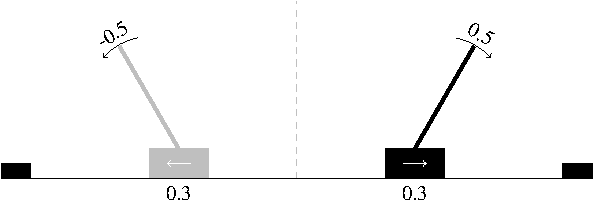
\includegraphics[width=4in]{figures/cart-pole}
  \caption{Cart Pole}
  \label{fig:cart-pole} 
\end{figure}

Let us study the capabilities of the continuous affine homomorphism
family, with the Cart Pole task as an example (\figref{fig:cart-pole}).
In this task, the agent must balance a pole on a cart without moving the
cart out of the boundaries; the only action the agent can perform is to
push the cart forward or backward with some force. The state variables
are the $x$ position of the agent, the angular displacement from the
vertical, and the linear and angular velocities of the cart and pole
respectively.

In a bounded domain, there is a single exact automorphism; a reflection
of all the state features about the centre of the track. This instance
is trivially captured by the continuous affine family, $A = -I$ and $b
= 0$. In an unbounded domain, however, the whole system is
translation-invariant, i.e. the $x$ position does not matter. In such
a case, $A$ could zero out the contribution of $x$, and $b$ translate
the system to any coordinate. This homomorphism is a reasonable
approximation even in bounded domains.

An interesting reduction we could study in this domain would be to
project the angular state space coordinates, and lift a policy from an
inverted pendulum. $A$ is simply the permutation matrix that shifts the
angular components to the first two features.
\end{example}

\section{Homomorphic Filters}
\label{sec:hf:homomorphic-filters}

% Exact symmetry -> Approximate symmetry
A number of factors make searching for exact homomorphisms impractical.
Rarely is the environment model exactly known, particularly in some
closed form that it can be exploited. Furthermore, exact homomorphisms
are extremely sensitive to noise, thus rendering them inapplicable to
any learnt models. Given these conditions, it is more prudent to search
for approximate homomorphisms. In this section, we describe an online
algorithm to find homomorphisms from the current environment, $\mdp$, to
an environment the agent has encountered before, $\mdp'$. We assume that
we have a model of $\mdp'$, but not of $\mdp$. 

% While experience from $\mdp'$ can be used to learn $\mdp$ more
% effectively, we can not rely on any model of $\mdp$ until there have
% been enough steps to obviate the need for it!

In principle, we would like to find a homomorphism that minimises the
expected difference between $x' \sim P_{\mdp}(x,a)$ and $\him{x'} \sim
P_{\mdp'}(h(x,a))$, as well as $R_{\mdp}(x,a)$ and $R_{\mdp'}(h(x,a))$.
To this end, we propose the following objective function,
\begin{eqnarray}
  C(h) &=& \int_{\states \times \actions} \ud x \ud a ~ C(h,x,a) \label{eq:hf:cost}\\
  C(h,x,a) &=& \half \E[ (\him{x'} - h(x'))^2 ] + \half \E[ (R_{\mdp'}(\him{x}) - R_{\mdp}(x))^2 ] \nonumber.
\end{eqnarray}

Without a model for $\mdp$, the above expectations can not be evaluated,
let alone minimised. However, we can use samples of $x$, $a$, $x'$ and
$r$ collected by the agent's interaction with the world to perform
stochastic gradient descent,
\begin{eqnarray*}
  h_{t+1} &\gets& h_{t} - \alpha \innerprod{\grad_h C(h,x,a)}{\homset} \\
  \grad_h C &=& \half \grad_h [ \Tr( K( h(x) ) ) + ( m( h(x) ) - h(x') )^2 + ( R(h(x')) - r )^2   ] \\ 
  \grad_h C &=& \half \grad \Tr( K(h(x)) )\cdot \grad_h h(x) + (m(h(x)) - h(x')) ( \grad m(h(x)) \cdot \grad_h h(x) - \grad_h h(x') )  \\
            &+& ( R(h(x')) - r ) \grad R( h(x') )\cdot \grad_h h(x').
\end{eqnarray*}
$m$ and $K$ are the mean and co-variance of $\mdp'$. Note that we
project the updates onto $\homset$, $\innerprod{\grad_h
C(h,x,a)}{\homset}$.

Finally, as $C(h)$ is in general a complex non-convex function, we
perform the stochastic gradient descent simultaneously on a number of
starting points, or particles. The algorithm is summarised in
\algoref{algo:homo-pf}. The $Q$-value at any point of the homomorphic
filter is computed as an expectation over each particle, with
probabilities proportional to $\exp(-\frac{C(\tilde{h}^j,x,a)}{\tau})$.

\begin{algorithm}[ht]
  \DontPrintSemicolon
  Initialise $M$ particles $h_0^{(i)}$ randomly from $\homset$ \;
  \While{ not converged }{
  \lForEach{particle $i$}{$\tilde{h}_{t+1}^i \gets h_{t}^i + \alpha \innerprod{\grad_h C}{\homset}$} \;
  \lForEach{particle $i$}{$h_{t+1}^i \sim \tilde{h}_{t+1}$ with probability $\propto \exp(-\frac{C(\tilde{h}^j,x,a)}{\tau})$}
  }
  \caption{Homomorphic Filtering}
  \label{algo:homo-pf}
\end{algorithm}

\subsection{Continuous Affine Homomorphisms}
One possible choice for $\homset$ is the set of affine transformations
between the state spaces, i.e. $h(x) = I_{m,n} A x + b$, where $m$ and
$n$ are dimensions of $\mdp'$ and $\mdp$ respectively, $A$ is an
arbitrary orthogonal matrix, and $b$ is an arbitrary translation. Below,
we derive the necessary update equations for this family of
homomorphisms,
\begin{align*}
  \diff{A_{ij}} h(x) &= I_{m,n} 1_i x_j  & \diff{A} f(h(x)) &= \grad f(h(x)) I_{m,n} x^T  \\
  \diff{b_i} h(x) &= 1_i & \diff{b} f(h(x)) &= \grad f(h(x)).
\end{align*}

\begin{eqnarray*}
  \diff{A} C &=& \half \grad \Tr( K(h(x)) ) x^T + \sum_i (m_i(h(x)) - h(x')) (\grad m_i(h(x)) \cdot I_{m,n}^T x^T - 1 \cdot I_{m,n}^T x'^T) \\
             &+& (R(h(x')) - r) \grad R( h(x') ) I_{m,n} x'^T \\
  \diff{b} C &=& \sum_i ( \half \grad K_i(h(x)) + ( m_i(h(x)) - h(x')) (\grad m_i(h(x)) - 1) ) \\
             &+& (R(h(x')) - r) \grad R( h(x') ).
\end{eqnarray*}

The new $A$ can be projected onto the set of orthogonal matrices, by
finding the nearest orthogonal matrix, $A (A^T A)^{-\half}$.

\section{Experimental Results}
\label{sec:hf:experiments}
% Experimental results

%Random orthogonal matrices were generated using Stewart's algorithm (1980).

We evaluated our algorithm on the Cart Pole domain. The domain
describes an agent that must balance a pole on a cart by applying
a linear force to the cart. The domain has four state variables,
$\theta$, the angular displacement of the pole from the vertical, $x$
the linear displacement of the cart from the center, and their
derivatives, $\dot{\theta}$ and $\dot{x}$. The linear force the agent
can apply is discretised into 4 actions. 

We used fitted Q-iteration with support vector regression through out
the experiments to learn the value function. We initially chose Gaussian
process regression to learn the domain models because it provided
a covariance function. However, despite the uniform noise in our
experiments, and hence independence from coordinates, the learnt models
did not accurately predict the variance, and led to greater variability
in performance.  We decided to omit the contribution of variance to the
gradient descent updates, and used the models learnt using support
vector regression for the remainder of the experiments for efficiency
reasons.

The Cart Pole domain has a single exact homomorphism which is a complete
reflection of the coordinates, and reversal of the forces applied. Since
the action space is discrete, we also added {\em an action permutation}
to each particle. Our algorithm found homomorphisms which a combination
of reflections of the angular components, and linear displacements of
cart along the track, both of which are intuitive. When the track on
which the cart moves is bounded, any two positions along the track,
except for mirror reflections, are {\em not} equivalent. However, the
difference in their values is reduces as the cart moves away from the
wall; in limiting case, when the track is unbounded, the $x$
displacement indeed does not matter. 

\begin{table}[hbtp]
%  \floatconts
  \centering
  \begin{tabular}{llll}
  \toprule
  \bfseries $l$, $m_p$, $m_c$ & \bfseries Using Original $\pi$ & \bfseries Using HF $\pi$ & \bfseries New Agent  \\
  \midrule
   $0.5$, $0.1$, $1.0$ & -11.003 & 1.612 & 2.079 \\
  \bottomrule
  \end{tabular}
  \caption{Lifted Policy on Perturbed Domain (Return after $1,600$ epochs)}
  \label{tbl:perturbed-values}
\end{table}

We perturbed the domain by changing some of its parameters (e.g. length
of the pole, masses, etc.), as well as by rotating the state space
coordinates, and observed the performance of the algorithm. We present
the return accumulated by the agent after $1,600$ epochs observations in
\autoref{tbl:perturbed-values}; in general, the lifted policy of the
homomorphic filter was competitive to a trained agent on the perturbed
domain, considerably better than the trained agent in the original
domain.

\begin{figure}
  \centering
  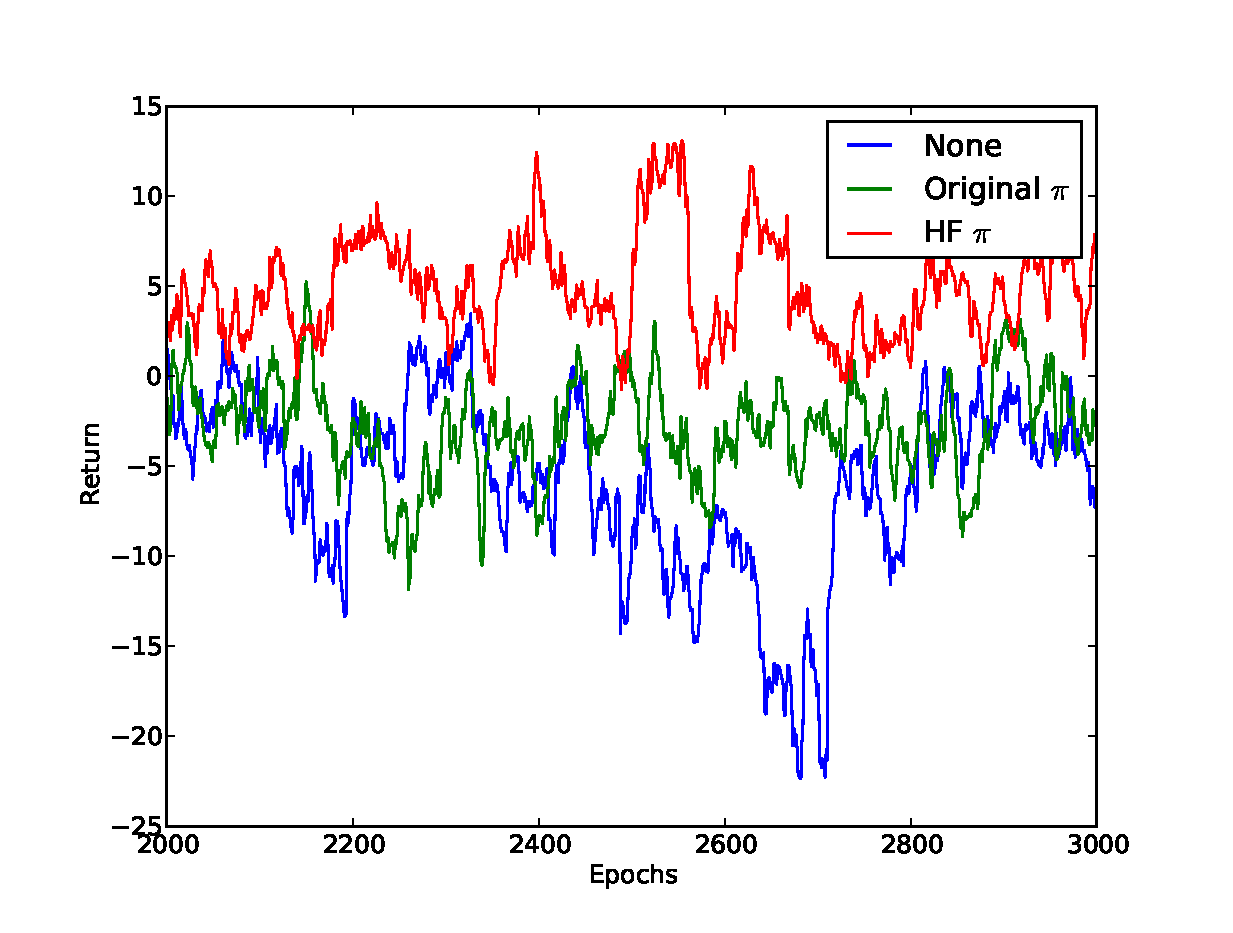
\includegraphics[width=4in]{figures/bootstrap}
  \caption{Bootstrapping Learning in a Perturbed Domain}
  \label{fig:bootstrap}
\end{figure}

We also evaluated the benefit of using the homomorphic filter to
bootstrap the agent using a slight variant of multiple model
reinforcement learning \citep{Doya2002}. Initially, the agent relies
more on the policy of the homomorphic filter, but as the agent's value
function estimate improves, it gradually begins to use its value
function more (\figref{fig:bootstrap}). We compared the performance of
an agent learning without any other model (None), with the policy learnt
in the original task (Original $\pi$), and the policy recommended by the
homomorphic filter (HF $\pi$). The agent using the homomorphic filter
significantly outperforms the other two agents. Note that the agent
using the original policy without any homomorphisms actually negatively
effects the learning of the agent.

%We also learnt a separate model of an inverted pendulum (without
%a cart), and provided the agent with this model.

